\chapter{รายละเอียดของงานที่ปฏิบัติ}
\label{chapter:related-theory}

ผู้ช่วยผู้ให้คำปรึกษาด้านความปลอดภัย (Associate Security Consultant) ทำหน้าที่ค้นหาช่องโหว่และทดสอบเจาะระบบในระบบสารสนเทศของลูกค้า และรายงานช่องโหว่กลับไปยังลูกค้าเพื่อให้ลูกค้าแก้ไข พร้อมทั้งประเมินความยากง่ายในการเจาะระบบ ความร้ายแรงที่จะเกิดขึ้นหากเกิดการเจาะระบบ และคำแนะนำในการแก้ไขช่องโหว่

ในบทนี้จะกล่าวถึงขึ้นตอนวิธีการเจาะระบบก่อน จากนั้นจะพูดถึงพื้นฐานของเว็บแอปพลิเคชัน ที่สามารถนำไปประยุกต์ใช้ในการเจาะระบบได้ ท้ายที่สุดจะพูดถึงเครื่องมือที่ช่วยอำนวยความสะดวกในการเจาะระบบ พร้อมทั้งสาธิตวิธีการเจาะระบบบนระบบเว็บแอปพลิเคชันจำลองที่มีช่องโหว่

\section{การทดสอบเจาะระบบ (Penetration Testing)}

ก่อนที่จะกล่าวถึงขึ้นตอนวิธีการค้นหาช่องโหว่ในระบบ ควรเข้าใจถึงคำว่าช่องโหว่ก่อน คำว่า “ช่องโหว่” (Vulnerability) นั้นหมายถึงข้อผิดพลาดของซอฟต์แวร์ (Bug) ที่สามารถใช้ในทางที่ไม่เหมาะสมเพื่อหลบหลีกระบบความปลอดภัยที่ใช้งานอยู่ขณะนั้น โดยที่วิธีการใช้งานช่องโหว่เพื่อเข้าถึงข้อมูลที่ไม่สมควรที่จะเข้าถึงได้ ในวงการ Cyber Security เรียกว่าการ “Exploit” หรือ “เจาะระบบ” นั่นเอง \cite{what-is-an-exploit} ซึ่งช่องโหว่ใด ๆ สามารถมีวิธีการเจาะระบบได้หลากหลายวิธี

ยกตัวอย่างเช่น ซอฟต์แวร์ของของลูกค้าอาจมีข้อผิดพลาดที่ทำให้อุปกรณ์มีปัญหาเมื่อมีการทำการใส่ข้อมูลนำเข้าประหลาด การอัพโหลดไฟล์รูปภาพที่ไม่ได้มีการตรวจสอบข้อมูลที่อยู่ในไฟล์รูป เพื่อยืนยันว่าเป็นไฟล์รูปจริง ๆ จึงทำให้สามารถแทรกโค้ดที่อันตรายไปในรูป แล้วสามารถส่งคำสั่งอันตรายขึ้นไปรันบนเครื่องได้ อาจจะทำให้มีผู้ที่ไม่หวังดีสามารถดึงข้อมูลที่เป็นความลับของลูกค้าออกไปได้ ซึ่งการที่ไม่มีการตรวจสอบชนิดของไฟล์นั้นคือช่องโหว่ที่ต้องแก้ไข (Vulnerability) ส่วนการแทรกโค้ดที่อันตรายไปในรูป แล้วสามารถส่งคำสั่งอันตรายขึ้นไปรันบนเครื่องลูกค้าได้ โดยที่ไม่ต้องยืนยันตัวตนนั้นคือวิธีการหลบหลีกระบบความปลอดภัยโดยใช้ข้อผิดพลาดของระบบ (Exploit)

เมื่อค้นพบช่องโหว่แล้ว ควรจะเจาะระบบเพื่อยืนยันว่าในระบบของลูกค้านั้นมีช่องโหว่นั้นอยู่จริง ๆ จากนั้นจึงรายงานการมีอยู่ของช่องโหว่ วิธีการเจาะระบบ และคำแนะนำในการแก้ไขให้แก่ลูกค้า ซึ่งกระบวนการเหล่านี้เรียกว่า “Penetration Testing” หรือเรียกสั้น ๆ ว่า “Pentest” ซึ่งบุคคลที่เจาะระบบเรียกว่า “Pentester”

ขั้นตอนวิธีการทำ Penetration Testing มีขั้นตอนดังต่อไปนี้

\subsection{Pre-engagement}

ก่อนที่จะเริ่มการทำ Penetration Testing ผู้ทดสอบเจาะระบบต้องพูดคุยทำความเข้าใจกับลูกค้าให้เข้าใจในสิ่งที่ตรงกัน ความเข้าใจที่คลาดเคลื่อนอาจทำให้เกิดความเสียหายกับระบบของลูกค้าได้ เช่น หน้าที่ของผู้เขียนจะต้องทดสอบหาช่องโหว่ของระบบของลูกค้า ซึ่งจะตรงกับช่วง Testing ในวงจรการพัฒนาซอฟต์แวร์ ซึ่งไม่ได้มีแค่บริษัทของผู้เขียนที่ใช้งานตัวระบบของลูกค้า ณ ขณะนั้น อาจจะมีบริษัทอื่นเข้ามาทดสอบ Functional Test ของระบบก็เป็นได้ ซึ่งทางลูกค้าจะแยก Environment ของระบบไว้ให้ทั้งฝั่ง Pentester และ Functional Test หากมีการสื่อสารผิดพลาดเกิดขึ้น ทำให้เราทดสอบเจาะระบบบนฝั่ง Functional Test แล้วระบบเกิดล่มขึ้นมา จะทำให้การทำงานของฝั่ง Funtional Test ช้าลง และส่งผลเสียแก่ลูกค้า เป็นต้น
ในขั้นตอนนี้ผู้ทดสอบเจาะระบบควรใช้เวลาเข้าใจการเหตุผลว่าทำไมลูกค้าถึงอยากให้มีการทดสอบเจาะระบบ คำถามที่สำคัญที่ควรถามแก่ลูกค้าได้แก่ เพราะอะไรถึงอยากให้มีการเจาะระบบ สิ่งที่กลัวที่สุดหากถูกเจาะระบบจากผู้ที่ไม่หวังดีคืออะไร มีระบบหรืออุปกรณ์อะไรที่ควรระมัดระวังในการทดสอบเจาะระบบหรือไม่ (เช่น อุปกรณ์ทางการแพทย์ เป็นต้น)
นอกจากนี้ยังมีสิ่งที่สำคัญอื่น ๆ อีกที่ต้องตกลงกันกับลูกค้า เช่น

\begin{enumerate}
	\item Scope ตัวระบบที่จะให้ทดสอบอยู่บน IP อะไร สามารถใช้ช่องโหว่ที่ทำให้ตัวระบบล่มจนไม่สามารถใช้งานได้หรือไม่ 
	\item Testing Window ลูกค้าอาจจะต้องการให้ทดสอบเพี่ยงแค่ในวันที่หรือช่วงเวลาที่กำหนดให้เท่านั้น
	\item Contact Information ควรจะติดต่อใครหากเกิดสิ่งร้ายแรงขึ้น สามารถติด่อได้ 24 ชั่วโมงหรือไม่ ต้องใช้การเข้ารหัสจดหมายอิเล็กทรอนิกส์หรือไม่
	\item Documentation เอกสารสำคัญที่กำหนดสิทธ์ให้เราทำการทดสอบเจาะระบบ ยิ่งถ้าตัวระบบไม่ใช่ของลูกค้าโดยตรง แต่เป็นคู้ค้าของลูกค้าอีกทีนึง และควรจำกัดความรับผิดชอบหากมีอะไรร้ายแรงเกิดขึ้น
	\item Payment Terms การแบ่งจายเงิน ลูกค้าจะจ่ายเงินอย่างไร เมื่อไหร่ และเท่าไหร่
	\item Non-Disclosure Agreement สัญญาปกปิดข้อมูลของลูกค้า
\end{enumerate}

\subsection{Information Gathering}

ในขั้นตอนนี้ผู้ทดสอบเจาะระบบจะค้นคว้าหาข้อมูลภาพรวมของระบบว่ามีซอฟต์แวร์อะไรกำลังทำงานอยู่บ้าง เวอร์ชั่นอะไร แล้วแต่ละซอฟท์แวร์นั้นมีช่องโหว่ที่เคยเกิดขึ้นมาบ้างหรือไม่ กระบวนการนี้สามารถทำได้โดยการใช้เครื่องมือที่ช่วยในการทำ Port Scan\cite{???} เช่น Nmap\cite{???} เป็นต้น เมื่อตรวจพบเจอ Port\cite{???}  ที่ถูกเปิดใช้อยู่หมายเลข 80, 443 สามารถคาดเดาได้ว่าเป็นระบบ Web Application (เนื่องจากเปิด Port 80 และ 443) โดยที่เราสามารถตรวจสอบเวอร์ชั่นของ Web Server ได้โดยดูจาก HTTP Response Header เป็นต้น

\subsection{Threat Modeling}

อ้างอิงจากข้อมูลที่ได้จากขึ้นตอน Information Gathering มาลองคิดดูว่าหากมีผู้ทีไม่หวังดีต้อง
การจะเจาะระบบ จะมีเหตุการณ์ใดเกิดขึ้นบ้าง และทรัพยากรขององค์กรส่วนใดที่จะได้รับผลกระทบ เช่น ถ้าลูกค้าผลิตซอฟต์แวร์ของตัวเอง ผู้ไม่หวังดีก็อยากจะเข้าถึง Source Code ของระบบนั้น แล้วนำข้อมูลไปขายให้กับบริษัทคู่แข่งของลูกค้า เป็นต้น จากนั้นจึงสร้างแผนทดสอบการเจาะระบบ

\subsection{Vulnerability Analysis}

ขึ้นตอนนี้จะเริ่มการค้นหาช่องโหว่จากตัวระบบของลูกค้าโดยตรง โดยสามารถใช้เครื่องมือช่วยค้นหาช่องโหว่ได้ก็ดี หรือค้นหาช่องโหว่ด้วยมือก็ดี ซึ่งจะมีตัวอย่างในบทที่ 3 แต่ทว่าเครื่องมืออาจจะเกิดผลบวกเทียมได้ ดังนั้นต้องมีการตรวจสอบด้วยมือทุก ๆ ช่องโหว่ที่ถูกพบเจอด้วยเครื่องมืออีกครั้งหนึ่ง

นอกจากนี้ผู้ทดสอบเจาะระบบยังสามารถค้นหา Exploit สำหรับซอฟท์แวร์เวอร์ชั่นนั้น ๆ ได้ตามฐานข้อมูลสาธารณะเช่น www.exploit-db.com\cite{???}  หรือ Metasploit Framework\cite{???} เป็นต้น (บางเวอร์ชั่นอาจจะมีช่องโหว่ก็ได้ หรือไม่มีช่องโหว่ก็เป็นได้) ซึ่งผู้ทดสอบเจาะระบบจะต้องมั่นใจว่า Exploit ที่ใช้จะสามารถเจาะระบบได้จริง

\subsection{Exploitation}

ขั้นตอนนี้ผู้ทดสอบเจาะระบบเจาะช่องโหว่ที่พบเจอด้วย Exploit ของช่องโหว่นั้น ๆ ซึ่งถ้าหากเป็นช่องโหว่ที่เกิดจาก bussiness logic หรือ functional logic ผู้ทดสอบเจาะระบบต้องสร้าง Exploit ขึ้นมาเอง เช่น แอปของธนาคารที่ใช้โอนเงินสามารถโอนเงินที่มีจำนวนติดลบได้ ดั้งนั้น Exploit ของเราก็คือ จำนวนเงินที่มีค่าติดลบ เป็นต้น 

\subsection{Post Exploitation}

ในบางช่องโหว่เมื่อเจาะระบบแล้วอาจจะสามารถควบคุมเครื่องแม่ข่ายของลูกค้าได้ ซึ่งเราสามารถใช้เครื่องแม่ข่ายนี้เข้าถึงระบบภายใน (Internal)\cite{???}  ของลูกค้าต่อไป เพื่อเพิ่มระดับความรุนแรงของช่องโหว่ขึ้นได้ เช่น หากเราสามารถควบคุมเครื่อง Web Server ของลูกค้าได้ และเครื่องนั้นสามารถติดต่อกับระบบฐานข้อมูลลูกค้าภายใน เราสามารถใช้เครื่อง Web Server นั้นเป็นเครื่องตัวกลาง (Pivot)\cite{???} ในการเข้าถึงระบบฐานข้อมูลลูกค้าภายในได้ เป็นต้น

\subsection{Reporting}

ขั้นตอนสุดท้ายของการทำ Penetration Testing คือการเขียนรายงานส่งลูกค้า โดยจะรายงานช่องโหว่ที่พบเจอ (Findings) ความร้ายแรงของช่องโหว่นั้น ๆ และคำแนะนำในการแก้ไข
รายงานจะแบ่งออกเป็น 2 ประเภทดังนี้

\subsubsection{Executive Summary}

รายงานชนิดนี้อธิบายถึงเป้าหมายในการหาช่องโหว่ และอธิบายผลกระทบของช่องโหว่ในภาพรวม โดยรายงานชนิดนี้เขียนเพื่อให้ผู้บริหารที่ดูแลโครงการ หรือผู้ที่ไม่มีความรู้เฉพาะด้านอ่านเช่น จะไม่ใช้ประโยคว่า “ผู้เจาะระบบได้ใช้ช่องโหว่รหัส MS08-067 เพื่อให้ได้ Shell” แต่จะใช้ประโยคที่สื่อถึงผลกระทบของช่องโหว่แทน “ผู้เจาะระบบสามารถอ่านจดหมายอิเล็กทรอนิกส์ของทุกคนในองค์กรได้” เป็นต้น

\subsubsection{Technical Report}

รายงานชนิดนี้จะลงลึกถึงรายละเอียดด้านเทคนิค โดยจะมีรายละเอียดตั้งแต่การทำ Information Gathering ไปจนถึง Post Exploitation พร้อมทั้งประเมินความยากง่ายของการเจาะ และผลกระทบที่จะเกิดในแต่ละช่องโหว่ รายงานชนิดนี้ผู้ที่อ่านคือผู้พัฒนาระบบ


เนื่องจากลูกค้าของบริษัทที่ผู้เขียนได้ไปฝึกงานต้องการทราบเพียงช่องโหว่ที่มีอยู่ในระบบสารสนเทศเท่านั้น บริษัทที่ผู้เขียนไปฝึกงานจึงไม่ได้ทำตามขั้นตอนด้านบนทั้งหมด  แต่ทำเพียงแค่ขั้นตอน Pre-Engagement, Vunerability Analysis, Exploitation และ Reporting  ยกตัวอย่าง ลูกค้าธนาคารแห่งหนึ่งจะเปิดตัวแอปพลิเคชันใหม่บนมือถือ โดยตัวแอปพลิเคชั่นจะเชื่อมต่อกับ RESTful API ของธนาคาร ทางลูกค้าจึงจ้างบริษัทไปค้นหาเพียงแค่ช่องโหว่บนบนแอปพลิเคชั่นและ RESTful API เท่านั้น ไม่ได้อยากทราบว่าจะเกิดผลกระทบอะไรกับระบบสารสนเทศทั้งธนาคารหลังจากมีการทำ Exploit ของแต่ละช่องโหว่ จึงทำให้ไม่มีขั้นตอน Threat Modelling และ Post Exploitation

สุดท้ายลูกค้าจะให้ข้อมูลรายละเอียดเกี่ยวกับระบบมาในขั้นตอน Pre-Engagement จึงทำให้ไม่มีขั้นตอน Information Gathering

\section{พื้นฐานสำหรับการทำ Penetration Testing บนเว็บแอปพลิเคชัน}

การค้นหาช่องโหว่ในเว็บแอปพลิเคชันนั้น จะหาได้อย่างง่ายดายหากผู้ทดสอบเจาะระบบมีความรู้ด้านการพัฒนาเว็บแอปพลิเคชันนั้น หรือเคยพัฒนาเว็บแอปพลิเคชันนั้นมาก่อน ในหัวข้อนี้จะเขียนถึงสิ่งที่ควรรู้เป็นพื้นฐานในการทดสอบเจาะระบบเว็บแอปพลิเคชัน โดยผู้ทดสอบเจาะระบบควรมีพื้นฐานในการใช้ Command Line การเขียนภาษาโปรแกรม และพื้นฐานระบบเครือข่ายมาก่อนด้วย

\subsection{HTTP Protocol}

Hyper Text Transfer Protocol (HTTP) คือมาตราฐานการส่งข้อมูลสื่อสิ่งพิมพ์ (รวมถึง HTML) ผ่านอินเทอร์เน็ต ซึ่ง HTTP  ใช้สถาปัตยกรรมแบบ Client-Server \cite{https://developer.mozilla.org/en-US/docs/Web/HTTP/Overview} ซึ่ง Client จะเริ่มต้นติดต่อ Server ก่อนเพื่อร้องขอข้อมูลที่ต้องการ (Request) จากนั้นจะรอให้ฝั่ง Server ตอบกลับ เมื่อ Server ตอบกลับ (Response) Client จะนำข้อมูลไปใช้งานต่อไป ถ้าหากตัว Client เป็น Web Browser เช่น Chrome หรือ Firefox เป็นต้น Browser ก็จะนำ Response ที่เป็น HTML ไปแสดงผลบนหน้าจอผู้ใช้ต่อไป \cite{https://developer.mozilla.org/en-US/docs/Web/HTTP/Messages} 

โดยปกติ HTTP ส่งข้อมูลผ่านเครือข่ายในรูปแบบที่ไม่ได้เข้ารหัส หากมีผู้ที่ไม่ประสงค์ดีดักจับข้อมูลระหว่างทาง แล้วมีการส่งข้อมูลรหัสผ่านยืนยันตัวตน หรือรหัสบัตรเครดิต ผู้ประสงค์ร้ายสามารถนำข้อมูลที่ได้มาไปสร้างความเสียหายแก่เราได้ จึงมีการพัฒนา HTTP ที่มีการเข้ารหัสขึ้นมาที่เรียกว่า HTTPs เรามักจะเห็นรูปแม่กุญแจ หรือคำว่า SECURE ข้างซ้ายของแถบ URL ของเว็บที่ใช้ HTTPs เพื่อบ่งบอกถึงข้อมูลที่รับส่งจากเว็บไซต์นี้ผ่านการเข้ารหัส ถึงแม้ว่าจะมีใครมาดักจับข้อมูล ก็จะไม่สามารถอ่านได้ เพราะข้อมูลนั้นถูกเข้ารหัสไว้อยู่

\begin{figure}[h]
	\centering
	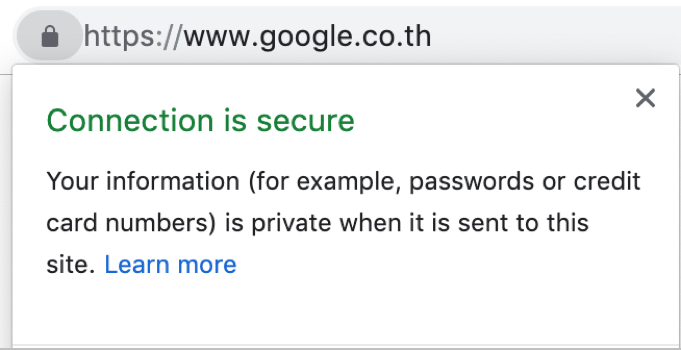
\includegraphics[width=0.6\columnwidth]{https.png}
	\caption{การเชื่อมต่อแบบ HTTPs บนเว็บไซต์ www.google.co.th}
	\label{Fig:https}
\end{figure}

\subsection{HTTP Cookie and Cookie Security}

เนื่องจาก HTTP เป็น Stateless Protocol ดังนั้น Server ไม่ทีทางรู้ได้ว่า แต่ละ Request ที่ส่งมานั้น มาจากผู้ใช้คนเดียวกันหรือไม่ ดังนั้นจึงมีสิ่งที่เรียกว่า Cookie เกิดขึ้น Cookie เป็น ข้อความรูปแบบ Key-Value ที่ Server ส่งให้กับ Client เพื่อที่ให้ Client แนบ Cookie นั้นมาทุก ๆ Request แล้ว Server จะได้รู้ว่าผู้ใช้คนใดเป็นคนส่งมา คล้าย ๆ กับการส่งจดหมายที่ต้องจ่าหน้าซองทุกครั้ง เพื่อที่จะได้รู้ว่าใครส่งมา \cite{https://developer.mozilla.org/en-US/docs/Web/HTTP/Cookies}

ในแต่ละ Domain จะมี Cookie แยกเป็นของตัวเอง และมีกฎในการอ่านเขียนดังนี้

\begin{enumerate}
	\item Cookie ที่ตั้งค่าโดย example.com สามารถถูกอ่านได้จากทุก ๆ Subdomain ของ example.com
	\item Cookie ที่ถูกเพิ่มโดย Subdomain สามารถอ่านได้โดย Subdomain นั้น และ Subdomain ของ Subdomain นั้น เช่น sub.example.com สามารถอ่าน Cookie ของ sub.example.com ได้ และ sub.example.com สามารถอ่าน Cookie ของ example.com ได้
	\item Subdomain สามารถตั้งค่า Cookie ของ Subdomain ของมันเอง และ Domain ที่เหนือกว่ามันได้ แต่ไม่สามารถตั้งค่า Cookie ของ Subdomain เครือญาติได้ เช่น foo.example.com ไม่สามารถ ตั้งค่า Cookie ของ bar.example.com ได้ แต่สามารถตั้งค่า Cookie ของ bar.foo.example.com และ example.com ได้
\end{enumerate}

นอกจากนี้ Server ควรตั้งค่า Secure Flag เพื่อให้ Cookie สามารถเข้าถึงผ่าน Https เท่านั้น และ HttpOnly Flag เพื่อไม่ให้ Javascript สามารถเข้าถึง Cookie ได้

\subsection{Web Framework}

Framework คือ ชุดคำสั่งหรือโปรแกรมที่ถูกวางโครงสร้างไว้ให้สำหรับนำไปพัฒนาต่อตามที่ต้องการ เปรียบเสมือนกับชุดตัวต่อ Lego® ที่มีเพียงแค่บล็อกสี่เหลี่ยม ซึ่งสามารถใช้ก่อสร้างกลายเป็นชิ้นงานตึกรามบ้านช่องต่าง ๆ ได้

การพัฒนาเว็บแอปพลิเคชันในปัจจุบันนั้นเป็นไปอย่างรวดเร็วตามความต้องการทางธุรกิจ ดังนั้นการใช้ Web Framework  จึงแพร่หลายเป็นอย่างมาก เพราะโครงสร้างพื้นฐานต่าง ๆ เช่น การเชื่อมต่อฐานข้อมูล การตรวจสอบความถูกต้องของข้อมูล ฯลฯ นั้นถูกจัดเตรียมมาใน Web Framework แล้วทั้งยังช่วยให้ผู้พัฒนาระบบหลีกเลี่ยงข้อผิดพลาดพลาดต่าง ๆ ที่จะเกิดขึ้นในการพัฒนาอีกด้วย

Web Framework ที่ผู้คนนิยมใช้ในปัจจุบันมีดังนี้

\begin{enumerate}
	\item Ruby on Rails (Ruby)
	\item Django (Python)
	\item Spring Boot (Java, Kotlin)
	\item Laravel (PHP)
\end{enumerate}

แต่ทว่าหากมีช่องโหว่ใน Web Framework แน่นอนว่าเว็บแอปพลิเคชันทั่วโลกที่ใช้งาน Web Framework นั้น ๆ ก็จะมีช่องโหว่ตามไปด้วย ดังนั้นการที่ทราบถึงชนิดของ Web Framework และ Version ที่ใช้จะช่วยให้หาช่องโหว่ได้ง่ายมากขึ้น

\subsection{Uniform Resource Locator}

Uniform Resource Locator (URL) เป็นเพียงแค่ชื่อที่อยู่ของทรัพยากรต่าง ๆ บนเว็บไซต์ ซึ่งแต่ละ URL จะชี้ไปยังทรัพยากรที่แตกต่างกัน เช่น ไฟล์ HTML, CSS, JavaScript หรือรูปภาพต่าง ๆ

ยกตัวอย่าง URL

\begin{lstlisting}
https://developer.mozilla.org:80/en-US/search?q=URL&key=value
\end{lstlisting}

สามารถอธิบายองค์ประกอบอย่างคร่าว ๆ ได้ดังนี้

\begin{enumerate}
	\item https:// หมายถึงโปรโตรคอลที่ตัว Browser ต้องใช้ในการเรียกหาทรัพยากร ซึ่งในที่นี้คือ HTTPs
	\item developer.mozilla.org คือชื่อ Domain ของเว็บไซต์ บ่งบอกว่ากำลังเชื่อมต่อกับ Web Server ตัวใดอยู่ ในที่นี้ developer.mozilla.org ชี้ไปยัง IP Address: 99.86.243.18
	\item :80 คือ Port เปรียบเสมือนกับประตูในการเข้าสู่เครื่องคอมพิวเตอร์ โดยที่แต่ละ Protocol จะมีการใช้ Port แตกต่างกันไป เช่น :80 สำหรับ HTTP และ :443 สำหรับ HTTPs โดยที่เราสามารถละเว้นการใส่ Port ได้สำหรับ HTTP กับ HTTPs หากทำงานอยู่บน :80 และ :443 ตามลำดับ
	\item /en-US/search คือ Path หมายถึง เส้นทางการเข้าถึงทรัพยากรในเครื่อง Server นั้น ๆ
	\item 5.	?q=URL\&key=value หมายถึงตัวแปรเพิ่มเติมที่ส่งให้ Web Server ไปประมวลผลข้อมูล โดยที่แต่ละตัวแปรจะถูกขั้นด้วยเครื่องหมาย \&
\end{enumerate}

\subsection{Binary to text encoding}

เป็นกระบวนการแปลงข้อมูลที่อยู่ในรูปของ Binary ให้อยู่ในรูปของตัวอักษรที่สามารถแสดงออกทางจอภาพได้ โดยทั่วไปแล้วในโลกของอินเทอร์เน็ตนิยมใช้ Base64 ในการแปลงรูปภาพให้เป็นตัวอักษรเพื่อที่จะสามารถใส่เข้าไปในไฟล์ HTML หรือ CSS ได้

ตัวอย่างการใช้อัลกอริทึม Base64 เพื่อการ encode รูปภาพดังต่อไปนี้

\begin{figure}[h]
	\centering
	
\includegraphics[width=0.2\columnwidth]{apple.png}
	\caption{โลโก้บริษัท แอปเปิ้ล จำกัด มหาชน}
	\label{Fig:apple.logo}
\end{figure}

ซึ่งภาพนี้เมื่อนำไปอ่านในรูปแบบของ Binary โดยโปรแกรม Hexdump \cite{???} จะได้ออกมาเป็นดังนี้ โดยจะขอแสดงเพียงบางส่วนเท่านั้น เนื่องจากไฟล์มีขนาดใหญ่

\begin{figure}[h]
	\centering
	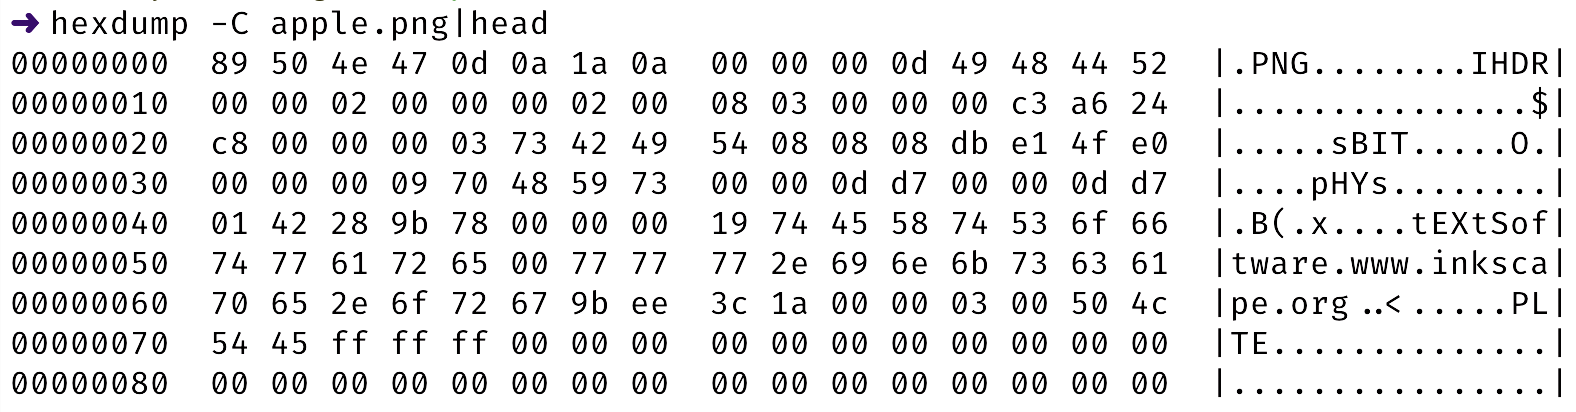
\includegraphics[width=1\columnwidth]{hexdump.png}
	\caption{ผลลัพธ์ของ Hexdump จากรูปโลโกด้านบน}
	\label{Fig:apple.logo.hex}
\end{figure}

และเมื่อนำภาพไป Encode ด้วย Base64 ได้ผลออกมาเป็นดังนี้ โดยจะขอแสดงเพียงผลลัพธ์ของ 112 Bytes แรกเท่านั้น

\begin{lstlisting}[numbers=none]
iVBORw0KGgoAAAANSUhEUgAAAZAAAAGQCAAAAACl1GkQAAAXp0lEQ
VR42u2dzVElyQ6FzyIjMkKhlBZa1OpagA0YgAVYgA04gAkYgAc4wB4L2GM
A61pkVKbeIusC3TPvTb+Z6arqRicmJnp6mo7gfg==
\end{lstlisting}

ด้วยข้อมูลในรูปแบบตัวอักษรนี้ (Text) ทำให้ง่ายต่อการใช้ส่งข้อมูลในโปรโตคอล HTTP ที่ไม่รองรับการส่งข้อมูลแบบ Binary หรือสามารถนำไปใช้เป็นรูปภาพใน HTML ได้โดยใช้ Tag ดังนี้

\begin{lstlisting}[numbers=none]
<img src="data:image/png;base64, iVBORw0KGgoAAAANSUhEUgAAAZAAAAGQCAAAAACl1GkQAAAXp0lEQ VR42u2dzVElyQ6FzyIjMkKhlBZa1OpagA0YgAVYgA04gAkYgAc4wB4L2GM A61pkVKbeIusC3TPvTb+Z6arqRicmJnp6mo7gfg==/>
\end{lstlisting}

\subsection{Encryption}

การเข้ารหัส (Encryption) ถือเป็นสิ่งที่ขาดไม่ได้ในระบบความปลอดภัย เพื่อที่ให้การสื่อสารของเรานั้น ไม่สามารถถูกดักไประหว่างทางแล้วถูกแอบอ่านได้

การเข้ารหัสมี 2 ประเภท ได้แก่

\begin{enumerate}
	\item การเข้ารหัสแบบกุญแจสมมาตร (Symmetric Key) เป็นกระบวนการเข้ารหัสที่ทั้งสองฝ่ายมีความลับร่วมกันอยู่ เมื่อดำเนินการส่งข้อมูลจริงจึงใช้ความลับนั้นมาถอดรหัสเพื่อให้ได้ข้อความที่อ่านออกกลับคืนมา ตัวอย่างของอัลกอริทึมการเข้ารหัสแบบกุญแจสมมาตร เช่น AES-256, Chacha-20, DES เป็นต้น โดยที่ AES-256 เป็นอัลกอริทึมที่นิยมมากที่สุดในการเข้ารหัสแบบกุญแจสมมาตร
	\item การเข้ารหัสแบบกุญแจอสมมาตร (Asymmetric Key) เป็นกระบวนการเข้ารหัสที่เปิดให้ผู้ส่งข้อมูลกับผู้รับข้อมูลสามารถใช้กุญแจคนละตัวกัน ที่สร้างมาคู่กันโดยเฉพาะ กล่าวคือ หากเข้ารหัสด้วยกุญแจใดก็ต้องถอดรหัสด้วยกุญแจอีกลูกหนึ่ง ตัวอย่างของอัลกอริทึมการเข้ารหัสแบบกุญแจอสมมาตร เช่น RSA (Rivest–Shamir–Adleman), ECC (Elliptic-curve cryptography) เป็นต้น
\end{enumerate}

\subsection{Hashing}

ทั้งนี้มีกระบวนการเข้ารหัสอีกรูปแบบหนึ่งที่มีคุณสมบัติสำคัญคือเมื่อเข้ารหัสไปแล้วไม่สามารถถอดรหัสได้อีก โดยผลลัพธ์ของการเข้ารหัสรูปแบบนี้เรียกว่า แฮช (Hash) โดยทั่วไปแล้วฟังก์ชันแฮชคือฟังก์ชันที่คืนค่าความยาวคงที่ (Fix Length) จากข้อมูลที่ความยาวเท่าไรก็ได้ (Variable Length)

ประโยชน์ที่สำคัญของการแฮช คือ ใช้ตรวจสอบความถูกต้องของข้อมูล เพราะการส่งข้อมูลจากต้นทางไปปลายทางมีโอกาสเสียหายได้ไม่ว่าจะมีคนแอบแก้ไข ความผิดพลาดของเครือข่าย หรือความผิดพลาดของมนุษย์ แฮชจึงเข้ามาช่วยแก้ปัญหานี้ด้วยการแฮชข้อมูลก่อนส่ง และหลังส่งแล้วมาเปรียบกัน ถ้าค่าแฮชตรงกัน หมายความว่าข้อมูลที่ส่งนั้นไม่ได้มีใครมาแก้ไข ยังคงเป็นค่าเดิม ตัวอย่างของอัลกอริทึมแฮช เช่น MD-5, SHA-1, SHA-256, Bcrypt เป็นต้น โดยที่ SHA-1 กับ MD-5 เลิกใช้แล้วเนื่องจากปัญหาด้านความปลอดภัย

ตัวอย่างการแฮชโดยอัลกอริทึมต่าง ๆ โดยผลลัพธ์ที่ได้เป็นเลขฐาน 16

% fold -w65
\begin{lstlisting}[numbers=none] 
md5(fox) = 2B95D1F09B8B66C5C43622A4D9EC9A04
md5(the fox) = 5595352FB8B1AF7F8241EB85A97BB2EB
sha1(fox) = FF0F0A8B656F0B44C26933ACD2E367B6C1211290
sha1(the fox) = D16A143050678D3AF5ACE6114DFCBF5BFA7C13C5
sha256(fox) = 776CB326AB0CD5F0A974C1B9606044D8485201F2DB19CF8E374
9BDEE5F36E200
sha256(the fox) = 812607450FD6745EDD149EE6EF07CF583B1C998E066D328
391FB1D7EA56FCEE8
\end{lstlisting}

\subsection{Authentication}

การรับรองตัวตนหรือยืนยันตัวตน (Authentication) กระทำเพื่อให้แน่ใจว่าเรากำลังติดต่อกับคนหรืออุปกรณ์ที่เราตั้งใจว่าจะติดต่อด้วยจริงหรือไม่

โดยทั่วไปแล้วกระบวนการยืนยันตัวตนมักจำแนกออกเป็น 3 ประเภท คือ

\begin{enumerate}
	\item เรารู้อะไร เราสามารถยืนยันตัวตนของคนที่คุยด้วยว่าเป็นตัวจริงหรือไม่ ด้วยการตรวจสอบว่าเขารู้ความลับบางอย่างที่รู้กันเฉพาะหรือไม่ ซึ่งนั่นก็คือรหัสผ่านที่เราใช้เป็นความลับเพื่อรับรองว่าเป็นตัวจริง 
	\item เรามีอะไร บางครั้งเราอาจใช้สิ่งของหรือหลักฐานเป็นเครื่องยืนยันตัวตน เช่น บัตรประชาชน หรือบัตรเครดิต สิ่งของเหล่านี้มักมีลักษณะเฉพาะคือมีเพียงชิ้นเดียวและอยู่ในความครอบครองของเจ้าของตัวจริงเพียงคนเดียวเท่านั้น
	\item เราเป็นใคร สิ่งที่เราเป็นสามารถใช้ยืนยันตัวตนของเราได้ เช่น ลายนิ้วมือ DNA หรือผู้ปกครองของผู้เขียนสามารถตามหาผู้เขียนในวัยเด็ก หัวเกรียน ๆ ได้โดยสังเกตุจากแผลเป็นบนศีรษะ
\end{enumerate}

โดยทั่วไปแล้วเราใช้เพียงกระบวนการใดกระบวนการหนึ่งข้างต้น ก็เพียงพอสำหรับการรับรองตัวตน แต่เราต้องเชื่อมั่นว่ากระบวนการนั้นมีประสิทธิภาพในการรับรองตัวตนจริง ๆ กล่าวคือต้องไม่มีใครสามารถปลอมบัตรประชาชนได้ หรือเราต้องไม่เคยบอกรหัสผ่านให้ใครรู้

\subsection{Authorization}

การให้อำนาจ (Authorization) กระบวนการนี้เมื่อเทียบกับชีวิตประจำวันคือการที่เราเข้าถึงพื้นที่ในอาคารต่าง ๆ ได้จำกัด หลังร้านอาหารอาจจะจำกัดเฉพาะพนักงานเข้าได้เท่านั้น ในขณะที่ลูกค้าทั่วไปจะต้องอยู่ในบริเวณที่น่าจัดไว้ หรือบริเวณชั้นผู้บริหารที่พนักงานทั่วไปไม่สามารถเข้าใช้งานได้ 

ในทางคอมพิวเตอร์เรามักจะเห็นกระบวนการให้อำนาจเช่นนี้อยู่ตลอดเวลา เช่น เว็บจำนวนมากที่ไม่เปิดให้ผู้ใช้แสดงความเห็นหรือโพสต์ข้อความใด ๆ ยกเว้นจะล็อกอินเสียก่อน การทำเช่นนี้คือการให้อำนาจกับผู้ใช้งานระบบที่แตกต่างกันไป

\subsection{Common Vulnerabilities and Exposure}

Common Vulnerabilities and Exposures (CVE) \cite{https://cve.mitre.org/} คือชื่อทางการของช่องโหว่ หากช่องโหว่นั้นเกิดบนซอฟท์แวร์ที่ใช้กันอยู่เป็นจำนวนมาก โดยมีรูปแบบเป็น CVE-YYYY-NNNN โดยที่ YYYY เป็นปี ค.ศ. ที่ค้นพบช่องโหว่ ส่วน NNNN แสดงลำดับในการค้นพบ ดังนั้น จะมีชื่อได้ 10,000 ชื่อ เช่น CVE-2016-5195  \cite{https://dirtycow.ninja/} แสดงว่า เป็นช่องโหว่ เกิดขึ้นปี 2016 และเป็นลำดับที่ 5159 ของปีนั้น

CVE-2016-5195 (Dirty Cow) เป็นช่องโหว่บน Linux Kernel ตั้งแต่เวอร์ชั่น 2.6.22 ซึ่งออกตั้งแต่ปี 2007 มีความร้ายแรงเป็นอย่างมาก ผู้มีสิทธิ์ต่ำสามารถยกระดับตนเองเป็นสิทธิ์สูงได้อย่างง่าย ดูโค้ดที่ใช้ Exploit ได้ที่นี่ https://www.exploit-db.com/exploits/40839

นอกจากนี้เราสามารถหา Exploit ของช่องโหว่ที่มี CVE ได้ตามอินเทอร์เน็ต แล้วนำมาทดลองเจาะระบบให้ลูกค้าได้ เพื่อเป็นการพิสูจน์ว่าระบบของลูกค้านั้นมีช่องโหว่จริง ๆ